La radiación ionizante es una herramienta moderna fundamental en el diagnostico y tratamiento de varias patologías. Su uso en medicina data desde la década de 1890, época en la que Roentgen reportó el descubrimiento de los rayos X y su capacidad de generar una imagen de los tejidos humanos internos de una forma efectiva, pero insegura por el desconocimiento parcial de los fenómenos involucrados. Gracias al desarrollo de la física detrás de estos fenómenos radiativos y al estudio de sus efectos sobre tejidos biológicos, se han logrado refinar estas herramientas para aplicaciones más sofisticadas como la radioterapia.\\

La eficiencia de estas herramientas en el diagnostico y tratamiento de enfermedades puede verse opacada por los grandes riesgos que se presentan cuando esta radiación no se aplica de manera segura. Por lo tanto, se hace necesario garantizar la seguridad en el uso de estos procedimientos, para lo cual es imprescindible la comprensión de los fenómenos físicos involucrados. Con este entendimiento es posible establecer protocolos de entrega de radiación y verificación de la misma que aseguren la máxima protección para todos los seres vivos que interactúan con ella. A continuación se expondrá un resumen de la teoría involucrada en estos procesos, así como algunos de los métodos que se usan en la actualidad para los propósitos antes mencionados.  \\

La radiación ionizante se refiere a aquellos haces de partículas con la capacidad de excitar o ionizar los átomos de la materia con la que interactúa. Para lograr este efecto se requieren energías de por lo menos 25 eV, que es la energía promedio con la cual están ligados al átomo los electrones en la capa de valencia. Por lo tanto, para que cierto haz de radiación electromagnética sea ionizante, este debe tener una longitud de onda no mayor a 320 nm, aproximadamente. \\

Los principales tipos de radiaciones ionizantes son los \textit{rayos} X, \textit{rayos }$\gamma$, haces de electrones libres, haces de neutrones y haces de partículas pesadas. Estos se pueden caracterizar por el tipo de partículas que son las portadoras de la energía y tienen propiedades particulares en cuanto a su poder de penetración.\\

Los rayos X y rayos $\gamma$ son radiación cuya energía es transportada por fotones. Los rayos X son radiación electromagnética emitida por partículas cargadas en transiciones atómicas, en cuyo caso se denominan rayos X característicos, o en procesos de Bremsstrahlung, en donde una partícula cargada es desacelerada por un campo columbiano de otra partícula cargada , por lo general tienen energías de entre  0.1 KeV hasta varios MeV dependiendo del proceso de generación. Los rayos $\gamma$ son radiación electromagnética producida por núcleos atómicos en un proceso de decaimiento radiactivo o procesos de aniquilación materia anti-materia, su magnitud de energía generalmente está en el rango de MeV.\\

En los tipos restantes de radiación ionizante, la energía es transportada por partículas con masa. En el caso de electrones, estos pueden ser producidos en un proceso nuclear, en cuyo caso se denominan rayos $\beta$ o en colisiones de partículas cargadas, en cuyo caso de denominan rayos $\delta$. Este tipo de haces pueden ser generados en aceleradores lineales(\textit{linacs}) para múltiples propósitos. Los haces de partículas pesadas son por lo general obtenidos en procesos de aceleración en campos columbianos o como decaimiento radiactivo, en tal caso la energía es transportada por núcleos atómicos pesados, como los rayos $\alpha$. Finalmente, los haces de neutrones son haces en los que la energía es transportada por estas partículas sin carga emitidas en procesos nucleares. \\

Todos estos tipos de radiación interactúan con la materia ionizandola, sin embargo, lo hacen de diferentes maneras. Se dice que un haz de radiación es de ionización directa si la energía que se imprime a la materia se transmite directamente mediante interacciones columbianas en la trayectoria de la partícula, como en el caso de los haces de partículas cargadas. Por otro lado, se dice que un haz de radiación es indirectamente ionizante si la energía se transmite a las partículas cargadas del medio mediante otro tipo de procesos que serán discutidos posteriormente, como es el caso de los rayos X y rayos $\gamma$, que transmiten su energía mediante tres procesos principales, el efecto fotoeléctrico, el efecto compton y la producción de pares.\\

       
\section{Medidas de radiación ionizante}
Teniendo en cuenta que la radiación ionizante es particularmente peligrosa en tejidos biológicos cuando no se tiene suficiente control sobre ella, es necesario desarrollar un sistema de medida que permita describir cuantitativamente los efectos en la que un haz con cierta energía interactúa con la materia que atraviesa.\\

En primer lugar, es posible caracterizar un haz es con su \textit{fluencia de partículas},denotada por $\Phi $, que se define como la cantidad diferencial dada por el cociente $dN$ por $da$, donde $dN$ es la cantidad esperada de partículas del haz que atraviesan una esfera imaginaria de sección transversal $da$.
\begin{equation}
	\Phi=\frac{dN}{da}.
\end{equation}   
Con esta cantidad se puede definir la \textit{densidad de flujo}, denotada por $\phi$ como la fluencia de partículas $\Phi$ por unidad de tiempo
\begin{equation}
	\phi=\frac{d\Phi}{dt}.
\end{equation}
Además, se define la \textit{fluencia de energía}, denotada por $\Psi$, como el valor esperado de energía de todas las partículas del haz que atraviesan una esfera imaginaria de sección transversal $da$.
\begin{equation}
	\Psi=\frac{dE}{da},
\end{equation}
y con esta se define la densidad de flujo de energía, denotada como $\psi$, como la fluencia de energía por unidad de tiempo
\begin{equation}
	\psi=\frac{d\Psi}{dt}.
\end{equation}
Por otro lado, es posible establecer unidades de medida para cuantificar la interacción de un haz con la materia. Las principales unidades de medida se presentan a continuación\\

\noindent
\textbf{Kerma($K$)}\\

Se define como la cantidad de energía cinética inicial de las partículas cargadas (electrones o positrones) que son liberadas por particulas sin carga (fotones) por unidad de masa
\begin{equation}
	K=\frac{dE_{tr}}{dm},
\end{equation}
el kerma tiene unidades de $J/Kg$, denominada tambien Gray (Gy), ($1J/Kg=1Gy$).
En el caso de un haz de fotones, es posible relacionar el kerma con la fluencia de energía mediante el \textit{coeficiente másico de transferencia de energía}, denotado por $(\mu_{tr}/\rho)_{E,Z}$, que es característico para cada material y la energía del haz, asi
\begin{equation}
	K=\Psi \left(\frac{\mu_{tr}}{\rho}\right)_{E,Z},
\end{equation} 
donde $\mu_{tr}$ es el \textit{coeficiente lineal de transferencia de energía}, con unidades $m^{-1}$ y $\rho$ es la densidad del material.\\

\noindent
\textbf{Dosis Absorbida($D$)}\\

La \textit{dosis absorbida}($D$) se define como el valor esperado de energía impartida en cierto material por unidad de masa
\begin{equation}
	D=\frac{d\epsilon}{dm},
\end{equation}
la cual también tiene unidades de Gray(Gy).\\

\noindent
\textbf{Dosis equivalente($H$)}\\

La \textit{dosis equivalente}($H$) se usa para incluir en la mediada los efectos que tiene la radiación sobre cierto tipo específico de tejido, mediante la inclusión de un factor de calidad $Q$
\begin{equation}
	H=Q\cdot D
\end{equation},
esta tiene unidades de Sievert(Sv), que tiene la misma unidades dimensionales que el Gray.\\

\noindent
\textbf{Exposición($X$)}\\

La \textit{exposición}($X$) se define como el valor absoluto de la carga de un signo producida cuando todos los electrones liberados por fotones en procesos de ionización son detenidos completamente en aire por unidad de masa
\begin{equation}
Q=\frac{dX}{dm},
\end{equation}
y tiene unidades de $C/Kg$.

\section{Interacción radiación materia}
Ahora, una vez determinadas las unidades con las que se medirá la radiación, es necesario establecer los mecanismos mediante los cuales esta interactúa con la materia y deposita energía en ella. Por lo tanto, a continuación se expondrán los procesos en los cuales los fotones depositan energía en los átomos y se presentará una manera de cuantificar este proceso numéricamente.  \\

Una partícula de un haz de radiación sin carga tiene alta probabilidad de pasar por una lámina delgada de algún materia sin perder energía, mientras que un haz de partículas cargadas probablemente pierda parte o la totalidad de su energía. Ambos procesos hacen parte importante del proceso de transmisión de energía a la materia por parte de un haz de radiación. En esta sección estudiaremos los procesos directos en los que los fotones depositan energía.\\

\noindent
\textbf{Atenuación exponencial($X$)}\\


Consideremos un haz mono-energético de partículas sin carga que incide perpendicularmente en la superficie de un material de espesor $L$. Si inicialmente existen $N_0$ partículas en el haz, después de atravesar el material alguna proporción de estos habrá sido absorbida en alguna de las diversas interacciones que pueden ocurrir con las partículas cargadas en el medio. En una primera aproximación, consideramos el caso ideal en que ninguna radiación secundaria es producida, es decir, las partículas del haz o bien son absorbidas completamente, o bien pasan a través sin perder nada de su energía.\\

Para dar cuenta de este efecto de absorción general mediante diferentes mecanismos, se propone el modelo de atenuación exponencial, en el que se modela el cambio en el numero de partículas en el haz $dN$ mediante la relación
\begin{equation}
	dN=-\mu N dl,
\end{equation}  
donde $\mu$ es denominado el \textit{coeficiente de atenuación lineal} y está asociado a la probabilidad de que una partícula del haz sea absorbida en su trayecto por una distancia $dl$. Además, si esta cantidad se divide por la densidad $\rho$ del medio de atenuación, se obtiene el coeficiente másico de atenuación $\mu/\rho$.\\

Integrando esta relación entre $0$ y el espesor $L$ del material, obtenemos la relación
\begin{equation}
	N=N_0 e^{-\mu L},
\end{equation}
que es denominada la ley de atenuación exponencial, que da cuenta del número de partículas que no fueron absorbidas por el medio en su recorrido por el material de espesor $L$.\\

Para determinar este coeficiente asociado a la probabilidad de absorción, es necesario estudiar los mecanismos principales en los que se transfiere o deposita energía de un haz de partículas sin carga. En el contexto de radioterapia, existen tres principales mecanismos de transmisión de energía  de fotones a partículas con masa. A continuación se relacionan estos y una descripción de cómo modifican este coeficiente de atenuación.\\

\noindent
\textbf{Dispersión elástica e ineslástica}\\

Los procesos de dispersión se dan cuando un fotón incidente con cierta energía interactúa directamente con el átomo y no es absorbido por este. Existen dos tipos de dispersión, la primera es la dispersión elástica o de Rayleigh, en la cual el fotón es dispersado elásticamente, es decir, con un traspaso esencialmente nulo de energía al átomo, solo es redireccionado un ángulo pequeño respecto a la dirección de incidencia. Una representación de este proceso se puede ver en la figura \ref{fig:rayleigh}.\\
\begin{figure}[H]
	\centering
	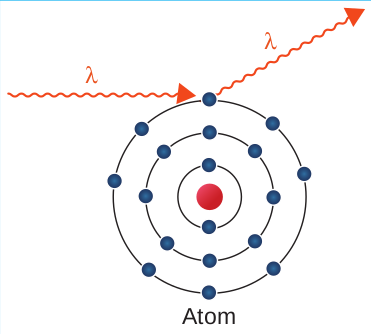
\includegraphics[width=0.7\linewidth]{images/rayleigh.png}
	\caption{Dispersión elástica}
	\label{fig:rayleigh}
\end{figure}
En este caso, el átomo se mueve solo lo suficiente para conservar el momento lineal. Por lo tanto, la contribución a la energía depositada por este proceso es nula.\\

Por otro lado, el segundo tipo de dispersión es el denominado \textit{efecto compton}. En este, un fotón incidente en un átomo interactua de forma no elástica con un electrón, que se asume libre y estacionario, impartiendo cierta energía en él. Para que este proceso suceda, la energía de ligadura del electrón al átomo debe ser mucho menor a la energía del fotón incidente. Este proceso se ve ilustrado en la figura \ref{fig:compton}.\\
\begin{figure}[H]
	\centering
	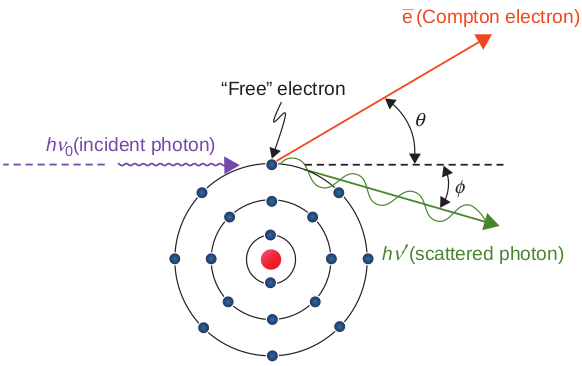
\includegraphics[width=0.7\linewidth]{images/compton.png}
	\caption{Dispersión no elástica- Efecto Compton}
	\label{fig:compton}
\end{figure}
En este proceso, el electrón es desligado del átomo y obtiene cierto momento en dirección $\theta$ con respecto a la dirección del fotón incidente. De la misma manera, el fotón es dispersado un ángulo $\phi$. \\

Este mecanismo puede ser estudiado desde la cinemática de la colisión de dos partículas relativistas. A partir de la conservación de energía y momento, es posible deducir las condiciones 
\begin{equation}
E=h \nu_{0} \frac{\alpha(1-\cos \phi)}{1+\alpha(1-\cos \phi)},
\end{equation}
\begin{equation}
h \nu^{\prime}=h \nu_{0}=\frac{1}{1+\alpha(1-\cos \phi)},
\end{equation}
\begin{equation}
\cot \theta=(1+\alpha) \tan \phi / 2,
\end{equation}
donde $h\nu_0$ es la energía del fotón incidente, $h\nu'$ es la energía del fotón dispersado, $E$ es la energía del electrón liberado y $\alpha=h\nu_0/m_0c^2$ con $m_0$ la masa en reposo del electrón. \\

Ahora, la probabilidad de que suceda un evento de este tipo puede calcularse mediante la sección eficaz del proceso. Esta viene dada por la fórmula de \text{Klein-Nishina}, que expresa que la sección eficaz diferencial para este proceso viene dada por
\begin{equation}
\frac{d_{e} \sigma}{d \Omega_{p}}=\frac{r_{0}^{2}}{2}\left(\frac{h \nu^{\prime}}{h \nu}\right)^{2}\left(\frac{h \nu}{h \nu^{\prime}}+\frac{h \nu^{\prime}}{h \nu}-\sin ^{2} \phi\right),
\end{equation}
donde $r_0=e^2/m_0c^2$ es el radio clásico del electrón.

\subsection{Efecto Fotoeléctrico}
\subsection{Producción de pares}
\section{Interacción de partículas cargadas}
\section{Fundamentos de dosimetria}
\subsection{Teoría de la cavidad}
\subsection{Camaras de ionización}
\section{Aceleradores en radioterapia}
\section{Peliculas radiocrómicas}
